\documentclass{article}

\usepackage{amsmath} % For math
\usepackage{amssymb} % For math
\usepackage{amsthm} % For math


\usepackage{graphicx} % For figures
\usepackage{subcaption} % For figure

\usepackage{float} % For figure placement

\usepackage{hyperref} % For links
\hypersetup{
    colorlinks,
    citecolor=black,
    filecolor=black,
    linkcolor=black,
    urlcolor=blue,
}
\usepackage{cleveref} % For references


\title{Math Basics}
\author{Mathias Balling Christiansen}
\date{Last updated: \today}

\begin{document}
\maketitle
\tableofcontents

\section{SinCosTan}
\hyperref[sec:SinCosTan relationer]{Relationer for SinCosTan}
\begin{center}
\begin{eqnarray*}
  \textbf{SOH} & \sin{\theta}&=\dfrac{\text{opposite}}{\text{hypotenuse}} \\
  \textbf{CAH} & \cos{\theta}&=\dfrac{\text{adjacent}}{\text{hypotenuse}} \\
  \textbf{TOA} & \tan{\theta}&=\dfrac{\text{opposite}}{\text{adjacent}}
\end{eqnarray*}

\input{Brøkregler}
\input{Kvadratsætninger}
\section{Potensregneregler}
\[a^r\cdot a^s=a^{r+s}\]

\[\frac{a^r}{a^s}=a^{r-s}\]

\[(a^r)^s=a^{r\cdot s}\]

\[(a\cdot b)^r=a^r\cdot b^r\]

\[\left (\frac{a}{b}\right )^r=\frac{a^r}{b^r}\]

\[a^0=1\]

\[a^{-r}=\frac{1}{a^r}\]

\[a^{-1}=\frac{1}{a}\]

\[\sqrt[r]{a}=a^{\frac{1}{r}}\]

\[\sqrt[s]{a^r}=a^{\frac{r}{s}}\]

\[\sqrt{a\cdot b}=\sqrt{a}\cdot \sqrt{b}\]

\[\sqrt{\frac{a}{b}}=\frac{\sqrt{a}}{\sqrt{b}}\]

\[\sqrt{a}=a^{\frac{1}{2}}\]
\section{Logaritmeregneregler}
\textbf{Husk formler fra matundervisning med log}
\[\log_{n}(a^x)=x\cdot \log_{n}(a)\]

\[\log_{n}(a\cdot b)=\log_{n}(a)+\log_{n}(b)\]

\[\log_{n}\left(\frac{a}{b}\right)=\log_{n}(a)-\log_{n}(b)\]

\[\log _n(a)=b \quad \Leftrightarrow \quad n^b=a\]

\[\log_{n}(n)=1\]

\[n^{\log_{n}(x)}=x\]

\[n^{\frac{a}{b}\cdot\log_n(x)}=\sqrt[b]{x^a}=x^{\frac{a}{b}}\]

\[n^{\log_n(x)\pm c}=x\cdot n^{\pm c}\]
Naturlig logaritme
\[\ln=\log_e\]

\[\ln(e)=1\]

\[e^{\ln(x)}=x\]

\[e^{\frac{a}{b}\cdot\ln(x)}=\sqrt[b]{x^a}=x^{\frac{a}{b}}\]

\[e^{\ln(x)\pm c}=x\cdot e^{\pm c}\]





\section{Vektorer i planen}
Koordinatsættet for $\vec{a}$
\[\vec{a}=a_1 \cdot \vec{i}+a_2 \cdot \vec{j}=\binom{a_1}{a_2} \]
Enhedsvektor
\[\vec{e}=\binom{\cos(v)}{\sin(v)}\]
Længden af $\vec{a}$
\[|\vec{a}|=\left|\binom{a_1}{a_2}\right|=\sqrt{a_1^2+a_2^2}\]
Multiplikation af $\vec{a}$ med tallet k
\[k\cdot\vec{a}=k\cdot\binom{a_1}{a_2}=\binom{k\cdot a_1}{k\cdot a_2}\]
Summen af to vektorere
\[\vec{a}+\vec{b}=\binom{a_1}{a_2}+\binom{b_1}{b_2}=\binom{a_1+b_1}{a_2+b_2}\]
Differensen af to vektorere
\[\vec{a}-\vec{b}=\binom{a_1}{a_2}-\binom{b_1}{b_2}=\binom{a_1-b_1}{a_2-b_2}\]
Koordinatsættet for $\overrightarrow{AB}$
\[\overrightarrow{AB}=\binom{x_2-x_1}{y_2-y_1}\]
Skalarproduktet (prikproduktet) af $\vec{a}$ og $\vec{b}$
\[\vec{a}\cdot\vec{b}=a_1b_1+a_2b_2\]

\[\vec{a}\cdot\vec{b}=|\vec{a}|\cdot|\vec{b}|\cdot\cos(v)\]

\[\cos(v)=\frac{\vec{a}\cdot\vec{b}}{|\vec{a}|\cdot|\vec{b}|}\]
Ortogonale vektorer
\[\vec{a}\cdot\vec{b}=0\quad\Leftrightarrow \quad \vec{a}\perp \vec{b}\]
Kvadratet på en vektor
\[\vec{a}\cdot\vec{a}=\vec{a}^2=|\vec{a}|^2\]
Projektion af $\vec{b}$ på $\vec{a}$
\[\vec{b}_a=\frac{\vec{a}\cdot\vec{b}}{|\vec{a}|^2}\cdot\vec{a}\]
Længden af projektionen
\[\vec{b}_a=\frac{|\vec{a}\cdot\vec{b}|}{|\vec{a}|}\]
Tværvektoren til $\vec{a}$
\[\hat{\vec{a}}=\widehat{\binom{a_1}{a_2}}=\binom{-a_2}{a_1}\]
Determinanten for vektorparret $(\vec{a},\vec{b})$
\[\det(\vec{a},\vec{b})=\hat{\vec{a}}\cdot\vec{b}=a_1b_2-a_2b_1=\begin{vmatrix}
    a_1&b_1  \\
    a_2& b_2
   \end{vmatrix}\]

\[\det(\vec{a},\vec{b})=|\vec{a}|\cdot|\vec{b}|\cdot\sin(v)\]
Parallelle vektorer
\[\det(\vec{a},\vec{b})=0 \quad\Leftrightarrow\quad \vec{a}\| \vec{b} \]
Arealet af parallelogrammet udspændt af $\vec{a}$ og $\vec{b}$
\[A=|\det(\vec{a},\vec{b})|\]



https://www.webmatematik.dk/lektioner/matematik-a/vektorfunktioner
\section{Vektorer i rummet}
Vektorprodukt (Krydsprodukt):
$$\vec{a}\times \vec{b} =
\begin{pmatrix}
\begin{vmatrix}a_{2}&b_{2}\\ a_{3}&b_{3}\end{vmatrix} \\
\\
\begin{vmatrix}a_{3}&b_{3}\\ a_{1}&b_{1}\end{vmatrix} \\
\\
\begin{vmatrix}a_{1}&b_{1}\\a_{2} &b_{2}\end{vmatrix} 
\end{pmatrix} =\begin{pmatrix}
a_2b_3-a_3b_2\\
a_3b_1-a_1b_3\\
a_1b_2-a_2b_1
\end{pmatrix} 
$$
Længden af vektorproduktet:
$$\left| \vec{a}\times \vec{b} \right|=\left| \vec{a}\right|\left| \vec{b} \right|\sin v$$
Længden af vektorproduktet er også lig arealet af det parallellogram der udspændes af $\vec{a}$ og $\vec{b}$
$$A=\left|\vec{a}\times \vec{b}\right|$$
Parameterfremstilling for linjen l gennem punktet:$P_0(x_0,y_0,z_0)$ med retningsvektor $\vec{r}=\begin{pmatrix}r_1 \\r_2\\r_3\end{pmatrix}$
$$\begin{pmatrix}x \\y\\z\end{pmatrix}=\begin{pmatrix}x_0 \\y_0\\z_0\end{pmatrix}+t\begin{pmatrix}r_1 \\r_2\\r_3\end{pmatrix}$$
Afstand fra punktet P til linjen l der går gennem punktet $P_0$ med retningsvektor $\vec{r}$
$$dist(P,l)=\frac{\left|\vec{r}\times \overrightarrow{P_0P}  \right|}{\left|\vec{r}\right|}$$
Ligningen for planen $\alpha$ gennem punktet $P_0 (x_0,y_0,z_0)$ med normalvektor $\vec{n}=\begin{pmatrix}a\\b\\c\end{pmatrix}$
$$\vec{n}\cdot\begin{pmatrix}x-x_0\\y-y_0 \\z-z_0\end{pmatrix}=0$$
$$a\cdot(x-x_0)+b\cdot(y-y_0)+c\cdot(z-z_0)=0$$
Afstand fra punktet $P(x_1,y_1,z_1)$ til planen $\alpha$ gennem punktet $P_0 (x_0,y_0,z_0)$ med normalvektor $\vec{n}=\begin{pmatrix}a\\b\\c\end{pmatrix}$
$$dist(P,\alpha)=\frac{\left| \vec{n}\cdot\begin{pmatrix}x_1-x_0\\y_1-y_0\\z_1-z_0\end{pmatrix} \right|}{\left|  \vec{n}\right|}$$
Afstand fra punktet $P(x_1,y_1,z_1)$ til planen $\alpha$ med ligningen: $ax+by+cz+d=0$
$$dist(P,\alpha)=\frac{\left|ax_1+by_1+cz_1+d  \right|}{\sqrt{a^2+b^2+c^2}}$$
Ligningen for en kugle med centrum $C(x_0,y_0,z_0)$ og radius r:
$$(x-x_0)^2+(y-y_0)^2+(z-z_0)^2=r^2$$


https://www.webmatematik.dk/lektioner/matematik-a/vektorer-i-3d
\section{Rummet}
Cartesian koordinater
$$(x,\;y,\;z)$$
Cylindrisk koordinater
$$[r,\theta,z]$$

$$x=r\cdot \cos \theta $$

$$y=r\cdot \sin \theta $$

$$z=z$$

$$r=\sqrt{x^2+y^2}$$

$$\tan \theta=\frac{y}{x}$$
Sfæriske koordinater
$$[R,\;\phi,\;\theta]$$

$$x=R\cdot \sin \phi \cos \theta$$

$$y=R\cdot \sin \phi \sin \theta$$

$$z=R\cdot \phi$$

$$R=\sqrt{x^2+y^2+z^2}$$

$$\tan \phi=\frac{\sqrt{x^2+y^2}}{z}$$

$$\tan \theta=\frac{y}{x}$$

\section{Complex Numbers}
Cartesian coordinate system
$$z=x+yi$$
$$w=a+bi$$
\begin{center}
    $a,b,x,y\in\mathbb{R}$ og $z,w\in\mathbb{C}$
\end{center}

$$i^2=-1$$

$$\left|  i\right|=1$$

$$\frac{1}{i}=-j$$

$$\arg{(i)}=\frac{\pi}{2}$$ 

$$Re(z)=x$$

$$Im(z)=y$$

$$w+z=(a+x)+(b+y)i$$

$$w-z=(a-x)+(b-y)i$$

$$wz=(a+bi)(x+yi)=(ax-by)+(ay+bx)i$$

$$\frac{w}{z}=\frac{a+ib}{x+iy}=\frac{ax+by+i(bx-ay)}{x^2+y^2}$$
Argand diagram:
\begin{center}
    \includegraphics[width=80mm]{Images/argand-diagram.png}
\end{center}
Modulus
$$\left|w\right|=M=r=\left|a+bi\right|=\sqrt{a^2+b^2}$$

$$\left|wz\right|=\left|w\right|\left|z\right|$$

$$\left|\frac{z}{w}\right|=\frac{\left| z \right|}{\left| w \right|}$$
Argument
$$\arg(w)=\theta$$

$$\theta=\tan^{-1}\left(\frac{b}{a}\right)\pm p\cdot\pi$$
$$p\in\left\{ -1,0,1 \right\} $$

$$\arg{(wz)}=\arg{(w)}+\arg{(z)}$$

$$\arg{\frac{z}{w}}=\arg{(z)}-\arg{(w)}$$
Polar representation
$$z=r\cdot\cos\theta+i\cdot r\cdot \sin{\theta}$$

$$z=r\cdot(\cos\theta+i\cdot \sin{\theta})$$

$$z=r\cdot e^{i\theta}$$
Konjugeret
$$\overline{w}=a-bi$$

$$\overline{w+z}=\overline{w}+\overline{z}$$

$$\overline{wz}=\overline{w}\cdot\overline{z}$$
De Moivre's Theorem
$$(\cos{\theta}+i\sin{\theta})^n=\cos{(n\theta)}+i\sin{(n\theta)}$$

$$e^z=e^{x+iy}=e^{x}e^{iy}=e^{x}(\cos {y}+i\sin{y})$$

$$r^n=(r\cdot e^{i\theta})^n=r^n\cdot e^{i\theta n}=r^n\cdot (\cos{(\theta n)+i\cdot\sin{(\theta n)}})$$

$$r^{\frac{p}{q}}=(r\cdot\cos{\theta+i\cdot\sin{\theta})^{\frac{p}{q}}}=r^{\frac{p}{q}}\cdot(\cos{(\frac{p}{q}\cdot\theta)}+i\cdot\sin{(\frac{p}{q}\cdot\theta)})$$
$$$$
$$$$
$$$$
$$$$

\section{Differentialligninger}

\section{Differential- og integralregning}
Definition af differentialkvotient
$$f'(x_0)=\lim_{h \to 0}\frac{f(x_0+h)-f(x_0)}{h} $$
Ligning for tangenten i punktet $P(x_0,f(x_0))$
$$y=f'(x_0)\cdot(x-x_0)+f(x_0)$$
Konstantreglen
$$(k\cdot f(x))'=k\cdot f'(x)$$
Sumreglen
$$(f(x)\pm g(x))'=f'(x)\pm g'(x)$$
Produktreglen
$$(f(x)\cdot g(x))'=f'(x)\cdot g(x)+f(x)\cdot g'(x)$$
Kvotientreglen
$$\left ( \frac{f(x)}{g(x)}\right )'=\frac{f'(x)\cdot g(x)-f(x)\cdot g'(x)}{(g(x))^2}$$
Kædereglen
$$(f(g(x)))'=f'(g(x))\cdot g'(x)$$
Regneregler for integration
$$\int f(x)dx=F(x)+c$$

$$\int k\cdot f( x)dx=k\cdot \int f(x)dx$$

$$\int f (x)\pm g( x)dx=\int  f(x)dx\pm \int g( x)dx$$

$$\int f(g (x))\cdot g'(x)dx=\int f(t)dt, \quad t=g(x)$$

$$\int_a ^b f(x)dx=[F(x)]_a ^b=F(b)-F(a)$$

$$\int_a ^b f(x)dx=\int_a ^c f(x)dx+\int_c ^b f(x)dx$$

$$\int_a^b k\cdot f( x)dx=k\cdot \int^b_a f(x)dx$$

$$\int^b_a f (x)\pm g( x)dx=\int^{b}_{a}  f(x)dx\pm \int_a^b g( x)dx$$

$$\int^b_a f(g (x))\cdot g'(x)dx=\int^{g(b)}_{g(a)} f(t)dt=[F(t)]^{g(b)}_{g(a)}=F(g(b)-F(g(a))$$

\section{Funktioner}
\section{Procent- og rentesregning}

\section{SinCosTan relationer}
\label{sec:SinCosTan relationer}
\begin{center}
    \bgroup
    \def\arraystretch{1.5}
    \begin{tabular}{cc}
        $\cos^2\cdot\sin^2=1^2$&$\tan{x}=\frac{\sin{x}}{\cos{x}}$
    \end{tabular}
    \egroup
    \end{center}



\begin{center}
    \bgroup
    \def\arraystretch{1.5}
        \begin{tabular}{p{5cm} p{4cm}}
            $\cos(x+2\pi)=\cos(x)$&$\sin(x+2\pi)=\sin(x)$\\
            $\cos(-x)=\cos(x)$&$\sin(-x)=-\sin(x)$\\
            $\cos(\pi-x)=-\cos(x)$&$\sin(\pi-x)=\sin(x)$
        \end{tabular}
    \egroup
\end{center}
\[\cos{(x+y)}=\cos{x}\cdot \cos{y}-\sin{x}\cdot\sin{y}\]
\[\cos{(x-y)}=\cos{x}\cdot \cos{y}+\sin{x}\cdot\sin{y}\]
\[\sin{(x+y)}=\cos{x}\cdot \sin{y}-\sin{x}\cdot\cos{y}\]
\[\sin{(x-y)}=\cos{x}\cdot \sin{y}+\sin{x}\cdot\cos{y}\]
\[\cos{(x)}^2-\sin{(x)}^2=\cos{(2x)}\]

\include{Integrationstabel}
\section{SI prefixes}
\begin{center}
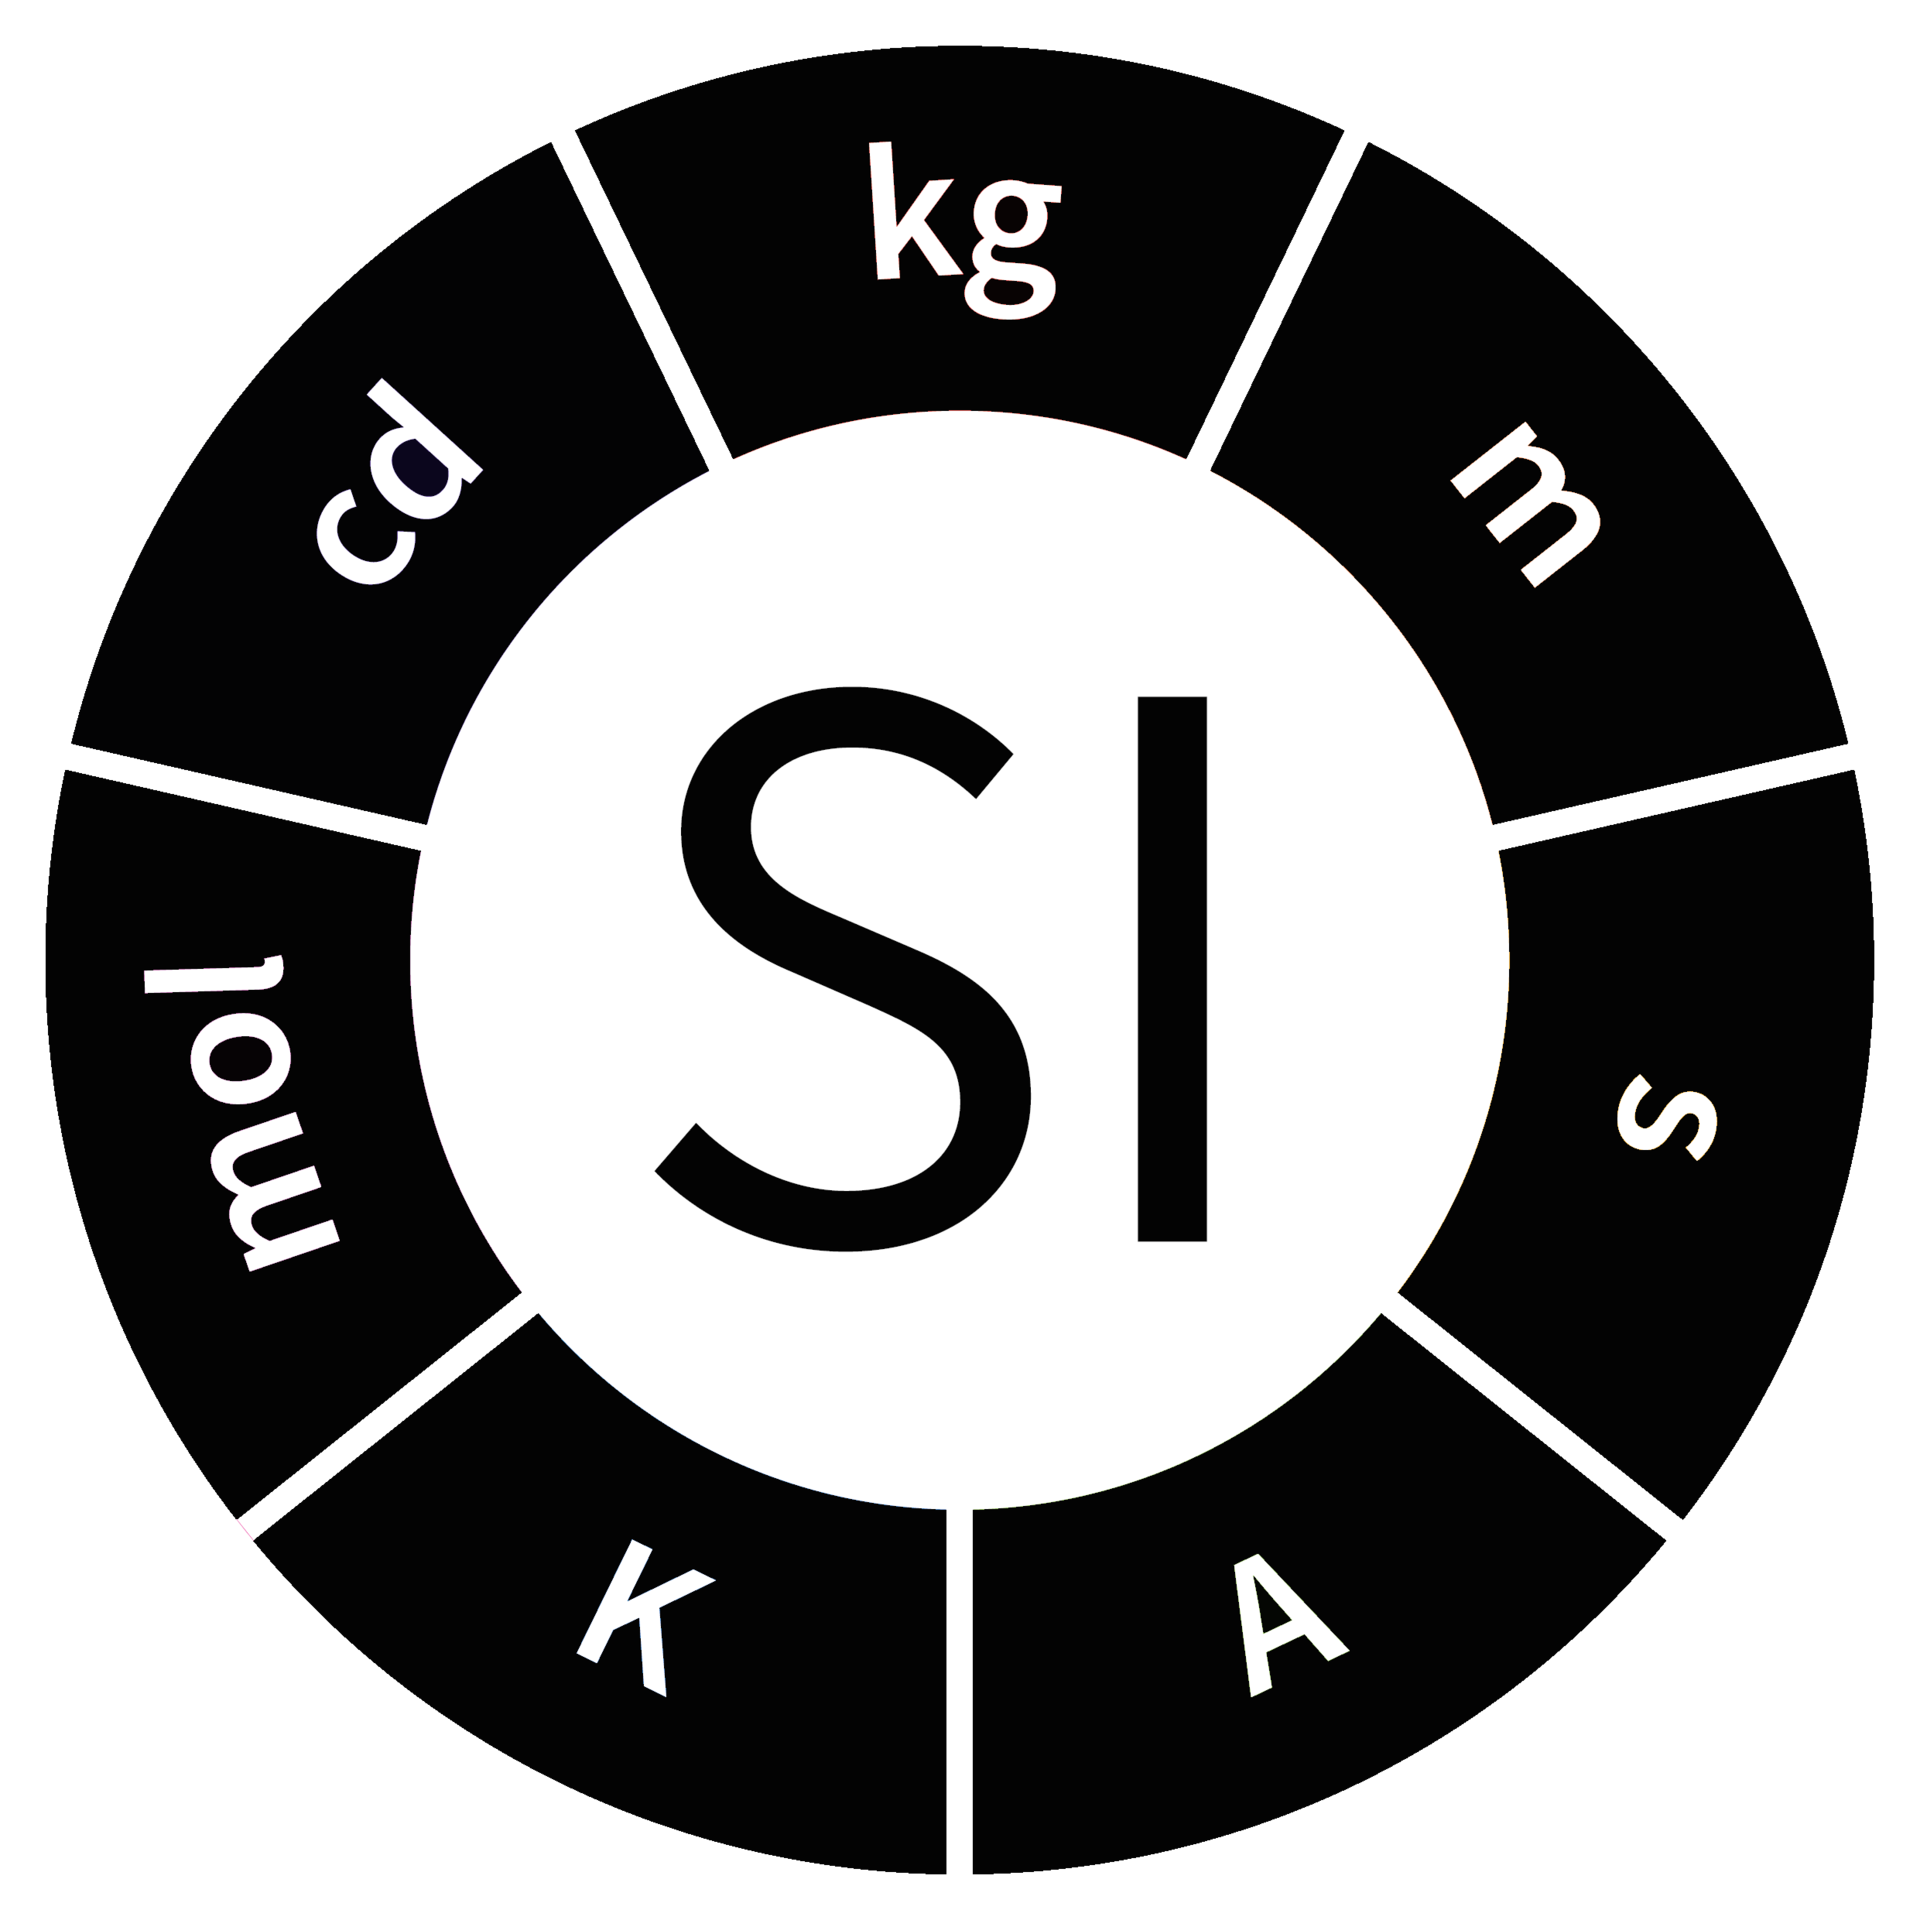
\includegraphics[width=70mm]{Images/SI-enheder.png}\\
\end{center}
Yotta (\textbf{Y}): $10^{24}$\\
Zetta (\textbf{Z}): $10^{21}$\\
Exa (\textbf{E}): $10^{18}$\\
Peta (\textbf{P}): $10^{15}$\\
Tera (\textbf{T}): $10^{12}$	\\
Giga (\textbf{G}): $10^9$	\\
Mega (\textbf{M}): $10^6$	\\
Kilo (\textbf{k}): $10^3$	\\
Hecto (\textbf{h}): $10^2$\\	
Deka (\textbf{da}): $10^1$\\	
Deci (\textbf{d}): $10^{-1}$\\
Centi (\textbf{c}): $10^{-2}$	\\
Milli (\textbf{m}): $10^{-3}$	\\
Micro (\textbf{µ}): $10^{-6}$	\\
Nano (\textbf{n}): $10^{-9}$	\\
Pico (\textbf{p}): $10^{-12}$	\\
Femto (\textbf{f}): $10^{-15}$\\	
Atto (\textbf{a}): $10^{-18}$	\\
Zepto (\textbf{z}): $10^{-21}$\\	
Yocto (\textbf{y}): $10^{-24}$\\

\end{center}

\end{document}
